\documentclass[aspectratio=169]{beamer}\usepackage[]{graphicx}\usepackage[]{xcolor}
% maxwidth is the original width if it is less than linewidth
% otherwise use linewidth (to make sure the graphics do not exceed the margin)
\makeatletter
\def\maxwidth{ %
  \ifdim\Gin@nat@width>\linewidth
    \linewidth
  \else
    \Gin@nat@width
  \fi
}
\makeatother

\definecolor{fgcolor}{rgb}{0.345, 0.345, 0.345}
\newcommand{\hlnum}[1]{\textcolor[rgb]{0.686,0.059,0.569}{#1}}%
\newcommand{\hlsng}[1]{\textcolor[rgb]{0.192,0.494,0.8}{#1}}%
\newcommand{\hlcom}[1]{\textcolor[rgb]{0.678,0.584,0.686}{\textit{#1}}}%
\newcommand{\hlopt}[1]{\textcolor[rgb]{0,0,0}{#1}}%
\newcommand{\hldef}[1]{\textcolor[rgb]{0.345,0.345,0.345}{#1}}%
\newcommand{\hlkwa}[1]{\textcolor[rgb]{0.161,0.373,0.58}{\textbf{#1}}}%
\newcommand{\hlkwb}[1]{\textcolor[rgb]{0.69,0.353,0.396}{#1}}%
\newcommand{\hlkwc}[1]{\textcolor[rgb]{0.333,0.667,0.333}{#1}}%
\newcommand{\hlkwd}[1]{\textcolor[rgb]{0.737,0.353,0.396}{\textbf{#1}}}%
\let\hlipl\hlkwb

\usepackage{framed}
\makeatletter
\newenvironment{kframe}{%
 \def\at@end@of@kframe{}%
 \ifinner\ifhmode%
  \def\at@end@of@kframe{\end{minipage}}%
  \begin{minipage}{\columnwidth}%
 \fi\fi%
 \def\FrameCommand##1{\hskip\@totalleftmargin \hskip-\fboxsep
 \colorbox{shadecolor}{##1}\hskip-\fboxsep
     % There is no \\@totalrightmargin, so:
     \hskip-\linewidth \hskip-\@totalleftmargin \hskip\columnwidth}%
 \MakeFramed {\advance\hsize-\width
   \@totalleftmargin\z@ \linewidth\hsize
   \@setminipage}}%
 {\par\unskip\endMakeFramed%
 \at@end@of@kframe}
\makeatother

\definecolor{shadecolor}{rgb}{.97, .97, .97}
\definecolor{messagecolor}{rgb}{0, 0, 0}
\definecolor{warningcolor}{rgb}{1, 0, 1}
\definecolor{errorcolor}{rgb}{1, 0, 0}
\newenvironment{knitrout}{}{} % an empty environment to be redefined in TeX

\usepackage{alltt}

% Set lecture number for later use


% Part common to all the lectures
\subtitle{MATH 2740 -- Mathematics of Data Science -- Lecture 08}
\author{\texorpdfstring{Julien Arino\newline\url{julien.arino@umanitoba.ca}}{Julien Arino}}
\institute{Department of Mathematics @ University of Manitoba}
\date{Fall 202X}

% Title of the lecture
\title{Matrix methods -- QR factorisation (2) \& SVD (1)}



\usetheme{default}
% Slide setup, colour independent

\usepackage{amsmath,amssymb,amsthm}
\usepackage[utf8]{inputenc}
\usepackage{colortbl}
\usepackage{bm}
\usepackage{xcolor}
\usepackage{dsfont}
\usepackage{setspace}
% To use \ding{234} and the like
\usepackage{pifont}
% To cross reference between slide files
\usepackage{zref-xr,zref-user}
% Use something like
% \zexternaldocument{fileI}
% in the tex files. And cite using \zref instead of \ref

% Cross-reference system - see CROSS-REFERENCE-SETUP.md for manual setup instructions
\usepackage{booktabs}
\usepackage{marvosym}
\usepackage{cancel}
%\usepackage{transparent}
% Make doi clickable in the bibliography?
\usepackage{doi}

\usepackage[T1]{fontenc}

\usepackage{longtable}

% For heavier titles
\usepackage{helvet} % Enables Helvetica font family


% Fields and the like
\def\IC{\mathbb{C}}
\def\IE{\mathbb{E}}
\def\IF{\mathbb{F}}
\def\II{\mathbb{I}}
\def\IJ{\mathbb{J}}
\def\IK{\mathbb{K}}
\def\IM{\mathbb{M}}
\def\IN{\mathbb{N}}
\def\IP{\mathbb{P}}
\def\IR{\mathbb{R}}
\newcommand{\IRplus}{\mathbb{R}_{\ge 0}}
\def\IZ{\mathbb{Z}}
\def\11{\mathds{1}}


% Bold lowercase
\def\ba{\bm{a}}
\def\bb{\bm{b}}
\def\bc{\bm{c}}
\def\bd{\bm{d}}
\def\be{\bm{e}}
\def\bf{\bm{f}}
\def\bg{\bm{g}}
\def\bh{\bm{h}}
\def\bi{\bm{i}}
\def\bj{\bm{j}}
\def\bk{\bm{k}}
\def\bn{\bm{n}}
\def\bp{\bm{p}}
\def\br{\bm{r}}
\def\bs{\bm{s}}
\def\bu{\bm{u}}
\def\bv{\bm{v}}
\def\bw{\bm{w}}
\def\bx{\bm{x}}
\def\by{\bm{y}}
\def\bz{\bm{z}}
\newcommand{\vect}[1]{\bm{#1}}

% Bold capitals
\def\bB{\bm{B}}
\def\bD{\bm{D}}
\def\bE{\bm{E}}
\def\bF{\bm{F}}
\def\bG{\bm{G}}
\def\bI{\bm{I}}
\def\bL{\bm{L}}
\def\bN{\bm{N}}
\def\bP{\bm{P}}
\def\bR{\bm{R}}
\def\bS{\bm{S}}
\def\bT{\bm{T}}
\def\bX{\bm{X}}

% Bold numbers
\def\b0{\bm{0}}

% Bold greek
\bmdefine{\bmu}{\bm{\mu}}
\def\bphi{\bm{\phi}}
\def\bvarphi{\bm{\varphi}}
\def\bPi{\bm{\Pi}}
\def\bGamma{\bm{\Gamma}}

% Bold red sentence
\def\boldred#1{{\color{red}\textbf{#1}}}
\def\defword#1{{\color{orange}\textbf{#1}}}

% Caligraphic letters
\def\A{\mathcal{A}}
\def\B{\mathcal{B}}
\def\C{\mathcal{C}}
\def\D{\mathcal{D}}
\def\E{\mathcal{E}}
\def\F{\mathcal{F}}
\def\G{\mathcal{G}}
\def\H{\mathcal{H}}
\def\I{\mathcal{I}}
\def\L{\mathcal{L}}
\def\M{\mathcal{M}}
\def\N{\mathcal{N}}
\def\P{\mathcal{P}}
\def\R{\mathcal{R}}
\def\S{\mathcal{S}}
\def\T{\mathcal{T}}
\def\U{\mathcal{U}}
\def\V{\mathcal{V}}

% Adding space for prime (') where needed
\def\pprime{\,'}
% Adding space for star (\star) where needed
\def\pstar{{\,\star}}

% tt font for code
\def\code#1{{\tt #1}}

% i.e., e.g.
\def\eg{\emph{e.g.}}
\def\ie{\emph{i.e.}}


% Operators and special symbols
\def\nbOne{{\mathchoice {\rm 1\mskip-4mu l} {\rm 1\mskip-4mu l}
{\rm 1\mskip-4.5mu l} {\rm 1\mskip-5mu l}}}
\def\cov{\ensuremath{\mathsf{cov}}}
\def\Var{\ensuremath{\mathsf{Var}\ }}
\def\Im{\textrm{Im}\;}
\def\Re{\textrm{Re}\;}
\def\det{\ensuremath{\mathsf{det}}}
\def\diag{\ensuremath{\mathsf{diag}}}
\def\nullspace{\ensuremath{\mathsf{null}}}
\def\nullity{\ensuremath{\mathsf{nullity}}}
\def\rank{\ensuremath{\mathsf{rank}}}
\def\range{\ensuremath{\mathsf{range}}}
\def\sgn{\ensuremath{\mathsf{sgn}}}
\def\Span{\ensuremath{\mathsf{span}}}
\def\tr{\ensuremath{\mathsf{tr}}}
\def\imply{$\Rightarrow$}
\def\restrictTo#1#2{\left.#1\right|_{#2}}
\newcommand{\parallelsum}{\mathbin{\!/\mkern-5mu/\!}}
\def\dsum{\mathop{\displaystyle \sum }}%
\def\dind#1#2{_{\substack{#1\\ #2}}}

\newcommand{\Qmatrix}[1]{%
  \begin{pmatrix}#1\end{pmatrix}%
}

\DeclareMathOperator{\GL}{GL}
\DeclareMathOperator{\Rel}{Re}
\def\Nt#1{\left|\!\left|\!\left|#1\right|\!\right|\!\right|}
\newcommand{\tripbar}{|\! |\! |}



% The beamer bullet (in base colour)
\def\bbullet{\leavevmode\usebeamertemplate{itemize item}\ }

% Theorems and the like
\newtheorem{proposition}[theorem]{Proposition}
\newtheorem{property}[theorem]{Property}
\newtheorem{importantproperty}[theorem]{Property}
\newtheorem{importanttheorem}[theorem]{Theorem}
%\newtheorem{lemma}[theorem]{Lemma}
%\newtheorem{corollary}[theorem]{Corollary}
\newtheorem{remark}[theorem]{Remark}
\setbeamertemplate{theorems}[numbered]
%\setbeamertemplate{theorems}[ams style]

%
%\usecolortheme{orchid}
%\usecolortheme{orchid}

\def\red{\color[rgb]{1,0,0}}
\def\blue{\color[rgb]{0,0,1}}
\def\green{\color[rgb]{0,1,0}}

% Fix skipping lines after items in the bibliography
\setbeamertemplate{bibliography entry title}{}
\setbeamertemplate{bibliography entry location}{}
\setbeamertemplate{bibliography entry note}{}

% Get rid of navigation stuff
\setbeamertemplate{navigation symbols}{}

% Set footline/header line
\setbeamertemplate{footline}
{%
\quad p. \insertpagenumber \quad--\quad \insertsection\vskip2pt
}
% \setbeamertemplate{headline}
% {%
% \quad\insertsection\hfill p. \insertpagenumber\quad\mbox{}\vskip2pt
% }


\makeatletter
\newlength\beamerleftmargin
\setlength\beamerleftmargin{\Gm@lmargin}
\makeatother

% Colours for special pages
\def\extraContent{yellow!20}


%%%%%%%%%%%%%%%%%
\usepackage{tikz}
\usetikzlibrary{shapes,arrows}
\usetikzlibrary{positioning}
\usetikzlibrary{shapes.symbols,shapes.callouts,patterns}
\usetikzlibrary{calc,fit}
\usetikzlibrary{backgrounds}
\usetikzlibrary{decorations.pathmorphing,fit,petri}
\usetikzlibrary{automata}
\usetikzlibrary{fadings}
\usetikzlibrary{patterns,hobby}
\usetikzlibrary{backgrounds,fit,petri}
\usetikzlibrary{tikzmark}

\usepackage{pgfplots}
\pgfplotsset{compat=1.6}
\pgfplotsset{ticks=none}

\usetikzlibrary{decorations.markings}
\usetikzlibrary{arrows.meta}
\tikzset{>=stealth}

% For tikz
\tikzstyle{cloud} = [draw, ellipse,fill=red!20, node distance=0.87cm,
minimum height=2em]
\tikzstyle{line} = [draw, -latex']


%%% For max frame images
\newenvironment{changemargin}[2]{%
\begin{list}{}{%
\setlength{\topsep}{0pt}%
\setlength{\leftmargin}{#1}%
\setlength{\rightmargin}{#2}%
\setlength{\listparindent}{\parindent}%
\setlength{\itemindent}{\parindent}%
\setlength{\parsep}{\parskip}%
}%
\item[]}{\end{list}}


% Make one image take up the entire slide content area in beamer,.:
% centered/centred full-screen image, with title:
% This uses the whole screen except for the 1cm border around it
% all. 128x96mm
\newcommand{\titledFrameImage}[2]{
\begin{frame}{#1}
%\begin{changemargin}{-1cm}{-1cm}
\begin{center}
\includegraphics[width=108mm,height=\textheight,keepaspectratio]{#2}
\end{center}
%\end{changemargin}
\end{frame}
}

% Make one image take up the entire slide content area in beamer.:
% centered/centred full-screen image, no title:
% This uses the whole screen except for the 1cm border around it
% all. 128x96mm
\newcommand{\plainFrameImage}[1]{
\begin{frame}[plain]
%\begin{changemargin}{-1cm}{-1cm}
\begin{center}
\includegraphics[width=108mm,height=76mm,keepaspectratio]{#1}
\end{center}
%\end{changemargin}
\end{frame}
}

% Make one image take up the entire slide area, including borders, in beamer.:
% centered/centred full-screen image, no title:
% This uses the entire whole screen
\newcommand{\maxFrameImage}[1]{
\begin{frame}[plain]
\begin{changemargin}{-1cm}{-1cm}
\begin{center}
\includegraphics[width=\paperwidth,height=\paperheight,keepaspectratio]
{#1}
\end{center}
\end{changemargin}
\end{frame}
}

% This uses the entire whole screen (to include in frame)
\newcommand{\maxFrameImageNoFrame}[1]{
\begin{changemargin}{-1cm}{-1cm}
\begin{center}
\includegraphics[width=\paperwidth,height=0.99\paperheight,keepaspectratio]
{#1}
\end{center}
\end{changemargin}
}

% Make one image take up the entire slide area, including borders, in beamer.:
% centered/centred full-screen image, no title:
% This uses the entire whole screen
\newcommand{\maxFrameImageColor}[2]{
\begin{frame}[plain]
\setbeamercolor{normal text}{bg=#2!20}
\begin{changemargin}{-1cm}{-1cm}
\begin{center}
\includegraphics[width=\paperwidth,height=\paperheight,keepaspectratio]
{#1}
\end{center}
\end{changemargin}
\end{frame}
}


\usepackage{tikz}
\usetikzlibrary{patterns,hobby,matrix}
\usepackage{pgfplots}
\pgfplotsset{compat=1.6}
\pgfplotsset{ticks=none}

\usetikzlibrary{backgrounds}
\usetikzlibrary{decorations.markings}
\usetikzlibrary{arrows.meta}
\tikzset{>=stealth}

\tikzset{
  clockwise arrows/.style={
    postaction={
      decorate,
      decoration={
        markings,
        mark=between positions 0.1 and 0.9 step 40pt with {\arrow{>}},
   }}}}


% New integrated section command: creates section and section slide
\newcommand{\Ssection}[2]{
\section{#1}
\begin{frame}[noframenumbering,plain]
  \begin{tikzpicture}[remember picture,overlay]
    \node[above right,inner sep=0pt,opacity=0.2] at (current page.south west)
    {
        \includegraphics[height=\paperheight,width=\paperwidth]{#2}
    };
  \end{tikzpicture}
  \setbeamercolor{section in toc}{fg=section_page_list_colour}
  \setbeamerfont{section in toc}{size=\Large,series=\bfseries}
  \setbeamertemplate{section in toc shaded}[default][60]
  \tableofcontents[
    currentsection,
    sectionstyle=show/shaded,
    subsectionstyle=show/hide/hide,
    subsubsectionstyle=hide/hide/hide]
\end{frame}
\addtocounter{page}{-1}
}

% New integrated section command with subsections: creates section and section slide showing subsections
\newcommand{\SsectionWithSubs}[2]{
\section{#1}
\begin{frame}[noframenumbering,plain]
  \begin{tikzpicture}[remember picture,overlay]
    \node[above right,inner sep=0pt,opacity=0.2] at (current page.south west)
    {
        \includegraphics[height=\paperheight,width=\paperwidth]{#2}
    };
  \end{tikzpicture}
  \setbeamercolor{section in toc}{fg=section_page_list_colour}
  \setbeamerfont{section in toc}{size=\Large,series=\bfseries}
  \setbeamertemplate{section in toc shaded}[default][60]
  \tableofcontents[
    currentsection,
    sectionstyle=show/hide,
    subsectionstyle=show/show/hide,
    subsubsectionstyle=hide/hide/hide]
\end{frame}
\addtocounter{page}{-1}
}

% New integrated subsection command: creates subsection and subsection slide
\newcommand{\Ssubsection}[2]{
\subsection{#1}
\begin{frame}[noframenumbering,plain]
  \begin{tikzpicture}[remember picture,overlay]
    \node[above right,inner sep=0pt,opacity=0.2] at (current page.south west)
    {
        \includegraphics[height=\paperheight,width=\paperwidth]{#2}
    };
  \end{tikzpicture}
  \setbeamercolor{section in toc}{fg=subsection_page_list_colour}
  \setbeamerfont{section in toc}{size=\Large,series=\bfseries}
  \setbeamertemplate{section in toc shaded}[default][60]
  \setbeamerfont{subsection in toc}{series=\bfseries}
  \setbeamertemplate{subsection in toc shaded}[default][50]
  \tableofcontents[
    currentsection,
    sectionstyle=show/hide,
    subsectionstyle=show/shaded/hide,
    subsubsectionstyle=hide/hide/hide]
\end{frame}
\addtocounter{page}{-1}
}

% New integrated subsubsection command: creates subsubsection and subsubsection slide
\newcommand{\Ssubsubsection}[2]{
\subsubsection{#1}
\begin{frame}[noframenumbering,plain]
  \begin{tikzpicture}[remember picture,overlay]
    \node[above right,inner sep=0pt,opacity=0.2] at (current page.south west)
    {
        \includegraphics[height=\paperheight,width=\paperwidth]{#2}
    };
  \end{tikzpicture}
  \setbeamercolor{section in toc}{fg=subsub_header_section}
  \setbeamerfont{section in toc}{size=\Large,series=\bfseries}
  \setbeamertemplate{section in toc shaded}[default][60]
  \setbeamerfont{subsection in toc}{series=\bfseries}
  \setbeamertemplate{subsection in toc shaded}[default][50]
  \setbeamertemplate{subsubsection in toc shaded}[default][50]
  \tableofcontents[
    currentsection,
    sectionstyle=show/hide,
    subsectionstyle=show/hide/hide,
    subsubsectionstyle=show/shaded/hide]
\end{frame}
\addtocounter{page}{-1}
}

% Legacy commands (kept for backward compatibility)
% Beginning of a section
\newcommand{\newSectionSlide}[1]{
\begin{frame}[noframenumbering,plain]
  \begin{tikzpicture}[remember picture,overlay]
    \node[above right,inner sep=0pt,opacity=0.2] at (current page.south west)
    {
        \includegraphics[height=\paperheight,width=\paperwidth]{#1}
    };
  \end{tikzpicture}
  \setbeamercolor{section in toc}{fg=section_page_list_colour}
  \setbeamerfont{section in toc}{size=\Large,series=\bfseries}
  \setbeamertemplate{section in toc shaded}[default][60]
  \tableofcontents[
    currentsection,
    sectionstyle=show/shaded,
    subsectionstyle=show/hide/hide,
    subsubsectionstyle=hide/hide/hide]
\end{frame}
\addtocounter{page}{-1}
}

% Beginning of a section in which we also show subsections
\newcommand{\newSectionWithSubsSlide}[1]{
	\begin{frame}[noframenumbering,plain]
		\begin{tikzpicture}[remember picture,overlay]
			\node[above right,inner sep=0pt,opacity=0.2] at (current page.south west)
			{
				\includegraphics[height=\paperheight,width=\paperwidth]{#1}
			};
		\end{tikzpicture}
		\setbeamercolor{section in toc}{fg=section_page_list_colour}
		\setbeamerfont{section in toc}{size=\Large,series=\bfseries}
		\setbeamertemplate{section in toc shaded}[default][60]
		\tableofcontents[
		currentsection,
		sectionstyle=show/hide,
		subsectionstyle=show/show/hide,
		subsubsectionstyle=hide/hide/hide]
	\end{frame}
	\addtocounter{page}{-1}
}

% Beginning of a subsection
\newcommand{\newSubSectionSlide}[1]{
\begin{frame}[noframenumbering,plain]
  \begin{tikzpicture}[remember picture,overlay]
    \node[above right,inner sep=0pt,opacity=0.2] at (current page.south west)
    {
        \includegraphics[height=\paperheight,width=\paperwidth]{#1}
    };
  \end{tikzpicture}
  \setbeamercolor{section in toc}{fg=subsection_page_list_colour}
  \setbeamerfont{section in toc}{size=\Large,series=\bfseries}
  \setbeamertemplate{section in toc shaded}[default][60]
  \setbeamerfont{subsection in toc}{series=\bfseries}
  \setbeamertemplate{subsection in toc shaded}[default][50]
  \tableofcontents[
    currentsection,
    sectionstyle=show/hide,
    subsectionstyle=show/shaded/hide,
    subsubsectionstyle=hide/hide/hide]
\end{frame}
\addtocounter{page}{-1}
}

% Beginning of a subsubsection
\newcommand{\newSubSubSectionSlide}[1]{
\begin{frame}[noframenumbering,plain]
  \begin{tikzpicture}[remember picture,overlay]
    \node[above right,inner sep=0pt,opacity=0.2] at (current page.south west)
    {
        \includegraphics[height=\paperheight,width=\paperwidth]{#1}
    };
  \end{tikzpicture}
  \setbeamercolor{section in toc}{fg=subsub_header_section}
  \setbeamerfont{section in toc}{size=\Large,series=\bfseries}
  \setbeamertemplate{section in toc shaded}[default][60]
  \setbeamerfont{subsection in toc}{series=\bfseries}
  \setbeamertemplate{subsection in toc shaded}[default][50]
  \setbeamertemplate{subsubsection in toc shaded}[default][50]
  \tableofcontents[
    currentsection,
    sectionstyle=show/hide,
    subsectionstyle=show/hide/hide,
    subsubsectionstyle=show/shaded/hide]
\end{frame}
\addtocounter{page}{-1}
}


   %%%%%%%%%%%
% To have links to parts in the outline
\makeatletter
\AtBeginPart{%
  \addtocontents{toc}{\protect\beamer@partintoc{\the\c@part}{\beamer@partnameshort}{\the\c@page}}%
}
%% number, shortname, page.
\providecommand\beamer@partintoc[3]{%
  \ifnum\c@tocdepth=-1\relax
    % requesting onlyparts.
    \makebox[6em]{Part #1:} \textcolor{green!30!blue}{\hyperlink{#2}{#2}}
    \par
  \fi
}
\define@key{beamertoc}{onlyparts}[]{%
  \c@tocdepth=-1\relax
}
\makeatother%

\newcommand{\nameofthepart}{}
\newcommand{\nupart}[1]%
    {   \part{#1}%
        \renewcommand{\nameofthepart}{#1}%
        {
          \setbeamercolor{background canvas}{bg=orange!50}
          \begin{frame}{#1}%\partpage 
          \hypertarget{\nameofthepart}{}\tableofcontents%
          \end{frame}
        }
    }

% This command creates a title page using TikZ only
\newcommand{\tikztitlepage}[1]{%
\begin{frame}[plain,noframenumbering]
  \begin{tikzpicture}[remember picture,overlay]
    % Background image
    \node[above right,inner sep=0pt,opacity=0.1] 
      at (current page.south west) 
      {\includegraphics[width=\paperwidth,height=\paperheight]{#1}};

    % University logo
    \node[anchor=north east, inner sep=5pt, opacity=0.9] 
      at (current page.north east)
      {
\includegraphics[width=0.2\textwidth]{FIGS-slides-admin/UM-logo-horizontal-CMYK.png}};
    
    % Title
    \node[anchor=center, align=center, 
          font=\fontsize{13}{15}\bfseries\color{UMbrown}, 
          text width=0.9\textwidth] 
          at ([yshift=2cm]current page.center)
          {\inserttitle};

      % Authors
      \node[anchor=center, align=center,
        font=\fontsize{10}{12}\bfseries\color{UMbrown},
        text width=0.7\textwidth]
        at ([yshift=0.8cm]current page.center)
        {\insertauthor};

      % Affiliation
      \node[anchor=north, align=center,
        font=\fontsize{9}{11}\color{UMbrown},
        text width=0.7\textwidth]
        at ([yshift=-0.2cm]current page.center)
        {\insertaffiliation};      
    % Date
    \node[anchor=north, align=center, 
          font=\fontsize{12}{16}\bfseries\color{UMbrown},
          text width=0.7\textwidth] 
          at ([yshift=0.2cm]current page.center)
          {\insertdate};

    % Land acknowledgement
    \node[anchor=south, align=justify, 
          font=\footnotesize, text=black, 
          text width=1.1\textwidth] 
          at ([yshift=0.5cm]current page.south)
          {The University of Manitoba campuses are located on original lands of Anishinaabeg, Ininew, Anisininew, Dakota and Dene peoples, and on the National Homeland of the Red River Métis.\\
          We respect the Treaties that were made on these territories, we acknowledge the harms and mistakes of the past, and we dedicate ourselves to move forward in partnership with Indigenous communities in a spirit of Reconciliation and collaboration.};
  \end{tikzpicture}
  \addtocounter{page}{-1}
\end{frame}
}
% The title page with figure
% \newcommand{\titlepagewithfigure}[1]{%
%   \begin{frame}[noframenumbering,plain]
%     \begin{tikzpicture}[remember picture,overlay]
%       \node[above right,inner sep=0pt,opacity=0.1] at (current page.south west)
%       {
%           \includegraphics[height=\paperheight,width=\paperwidth]{#1}
%       };
%       \node[anchor=north east,
%       inner sep=5pt,
%       opacity=0.9] at (current page.north east)
%       {
%           
\includegraphics[width=0.2\textwidth]{FIGS-slides-admin/UM-logo-horizontal-CMYK.png}
%       };
%       \node[anchor=south, 
%       align=justify, 
%       text=black, 
%       text width=1.1\textwidth,
%       font=\footnotesize]  (land_acknowledgement)
%       at (current page.south) 
%       {The University of Manitoba campuses are located on original lands of Anishinaabeg, Ininew, Anisininew, Dakota and Dene peoples, and on the National Homeland of the Red River Métis.
%       We respect the Treaties that were made on these territories, we acknowledge the harms and mistakes of the past, and we dedicate ourselves to move forward in partnership with Indigenous communities in a spirit of Reconciliation and collaboration.};  
%       % \node[align=center, anchor=south,
%       % above=0.5cm of land_acknowledgement,
%       % text=black,
%       % font=\bfseries] {\insertdate};
%   \end{tikzpicture}
%   \setbeamercolor{title}{fg=title_page_title_colour}
%   \setbeamerfont{title}{size=\Large,series=\bfseries}
%   \setbeamercolor{author}{fg=title_page_author_colour}
%   \setbeamerfont{author}{size=\large,series=\bfseries}
%   \setbeamercolor{institute}{fg=title_page_institute_colour}
%   \setbeamerfont{institute}{size=\large,series=\bfseries}
%   \setbeamercolor{date}{fg=title_page_date_colour}
%   \setbeamerfont{date}{series=\bfseries}
% 	\titlepage
% \end{frame}
% \addtocounter{page}{-1}
% }

\newcommand{\titlepagewithfigure}[1]{%
  \begin{frame}[noframenumbering,plain]
    \begin{tikzpicture}[remember picture,overlay]
      \node[above right,inner sep=0pt,opacity=0.1] at (current page.south west)
      {
          \includegraphics[height=\paperheight,width=\paperwidth]{#1}
      };
      \node[anchor=north east,
      inner sep=5pt,
      opacity=0.9] at (current page.north east)
      {
          
\includegraphics[width=0.2\textwidth]{FIGS-slides-admin/UM-logo-horizontal-CMYK.png}
      };
      \node[anchor=south, 
      align=justify, 
      text=black, 
      text width=1.1\textwidth,
      font=\footnotesize]  (land_acknowledgement)
      at (current page.south) 
      {The University of Manitoba campuses are located on original lands of Anishinaabeg, Ininew, Anisininew, Dakota and Dene peoples, and on the National Homeland of the Red River Métis.
      We respect the Treaties that were made on these territories, we acknowledge the harms and mistakes of the past, and we dedicate ourselves to move forward in partnership with Indigenous communities in a spirit of Reconciliation and collaboration.};  
      % \node[align=center, anchor=south,
      % above=0.5cm of land_acknowledgement,
      % text=black,
      % font=\bfseries] {\insertdate};
  \end{tikzpicture}
  \setbeamercolor{title}{fg=title_page_title_colour}
  \setbeamerfont{title}{size=\Large,series=\bfseries,family=\usefont{T1}{phv}{b}{n}}
  \setbeamercolor{author}{fg=title_page_author_colour}
  \setbeamerfont{author}{size=\large,series=\bfseries,family=\usefont{T1}{phv}{b}{n}}
  \setbeamercolor{institute}{fg=title_page_institute_colour}
  \setbeamerfont{institute}{size=\large,series=\bfseries,family=\usefont{T1}{phv}{b}{n}}
  \setbeamercolor{date}{fg=title_page_date_colour}
  \setbeamerfont{date}{series=\bfseries,family=\usefont{T1}{phv}{b}{n}}
	\titlepage
\end{frame}
\addtocounter{page}{-1}
}
% The outline page, with figure
% \newcommand{\outlinepage}[1]{%
% \begin{frame}[noframenumbering,plain]
%   \begin{tikzpicture}[remember picture,overlay]
%     \node[above right,inner sep=0pt,opacity=0.2] at (current page.south west)
%     {
%         \includegraphics[height=\paperheight,width=\paperwidth]{#1}
%     };
%   \end{tikzpicture}
%   \setbeamercolor{section in toc}{fg=outline_page_list_colour}
%   \setbeamerfont{section in toc}{size=\Large,series=\bfseries,family=\sffamily}
%   \frametitle{\textcolor{outline_page_title_colour}{\LARGE\bfseries Outline}}
%   \tableofcontents[hideallsubsections]
% \end{frame}
% \addtocounter{page}{-1}
% }
% The outline page, with figure
\newcommand{\outlinepage}[1]{%
\begin{frame}[noframenumbering,plain]
  \begin{tikzpicture}[remember picture,overlay]
    \node[above right,inner sep=0pt,opacity=0.2] at (current page.south west)
    {
        \includegraphics[height=\paperheight,width=\paperwidth]{#1}
    };
  \end{tikzpicture}
  \setbeamercolor{section in toc}{fg=outline_page_list_colour}
  % Use Helvetica Bold only for the outline slide TOC
  \setbeamerfont{section in toc}{size=\Large,family=\usefont{T1}{phv}{b}{n}}
  % Use Helvetica Bold for the outline title
  \frametitle{\textcolor{outline_page_title_colour}{\usefont{T1}{phv}{b}{n}\LARGE Outline}}
  \tableofcontents[hideallsubsections]
\end{frame}
\addtocounter{page}{-1}
}


%\let\oldsection\section
%\renewcommand{\section}[2]{\oldsection[#1]\newSectionSlide[#2]}


%%%%%%%%%%%%%%%%%%%%%
% CUSTOM SLIDE BACKGROUNDS
%%%%%%%%%%%%%%%%%%%%%
% Define custom background templates for different colors
\defbeamertemplate*{background canvas}{blue}{%
  \color{blue!15}\vrule width\paperwidth height\paperheight%
}
\defbeamertemplate*{background canvas}{green}{%
  \color{green!15}\vrule width\paperwidth height\paperheight%
}
\defbeamertemplate*{background canvas}{red}{%
  \color{red!15}\vrule width\paperwidth height\paperheight%
}
\defbeamertemplate*{background canvas}{yellow}{%
  \color{yellow!20}\vrule width\paperwidth height\paperheight%
}
\defbeamertemplate*{background canvas}{purple}{%
  \color{purple!15}\vrule width\paperwidth height\paperheight%
}
\defbeamertemplate*{background canvas}{orange}{%
  \color{orange!20}\vrule width\paperwidth height\paperheight%
}

% Define keys for the different background options
\makeatletter
\define@key{beamerframe}{blue}[true]{\setbeamertemplate{background canvas}[blue]}
\define@key{beamerframe}{green}[true]{\setbeamertemplate{background canvas}[green]}
\define@key{beamerframe}{red}[true]{\setbeamertemplate{background canvas}[red]}
\define@key{beamerframe}{yellow}[true]{\setbeamertemplate{background canvas}[yellow]}
\define@key{beamerframe}{purple}[true]{\setbeamertemplate{background canvas}[purple]}
\define@key{beamerframe}{orange}[true]{\setbeamertemplate{background canvas}[orange]}
\makeatother

% Reset to normal background for all frames by default
\BeforeBeginEnvironment{frame}{\setbeamertemplate{background canvas}[default]}

\newcommand{\punnett}[2]{
    \begin{center}
    \renewcommand{\arraystretch}{1.5} % Add space to rows
    \begin{tabular}{|c c | c|c|}
        \multicolumn{2}{c}{} & \multicolumn{2}{c}{\textbf{Father}} \\
        \multicolumn{2}{c}{} & #1 \\ \hline
        #2
    \end{tabular}
    \end{center}
}

% Colour definitions for Punnett squares
\usepackage{multirow}
\usepackage{colortbl}
\definecolor{punnettorange}{HTML}{F8C471} % A soft orange
\definecolor{punnettblack}{HTML}{BFC9CA} % A light grey for black
\definecolor{punnetttortie}{HTML}{E59866} % A brownish orange for tortie


\usetikzlibrary{positioning, decorations.pathreplacing, arrows.meta}

% --- TIKZ STYLES FOR CAT DIAGRAMS ---
\tikzset{
    % This is the main placeholder style for the cat images
    catnode/.style={
        draw, 
        rectangle, 
        rounded corners, 
        minimum height=1.5cm, 
        minimum width=2.5cm, 
        align=center, 
        font=\small\bfseries
    },
    % Allele styles (the X and Y at the top/side)
    allele/.style={font=\Large\bfseries},
    female/.style={allele, color=purple!80!black},
    male/.style={allele, color=blue!80!black},
    % --- Placeholder styles for different cats ---
    % YOU CAN REPLACE THE CONTENTS OF THESE NODES WITH YOUR IMAGES
    orange_cat/.style={
        catnode, 
        fill=orange!30, 
        text=black
    },
    black_cat/.style={
        catnode, 
        fill=black!70, 
        text=white
    },
    tortie_cat/.style={
        catnode, 
        fill=orange!50!black, % A mix for tortoiseshell
        text=white
    }
}

\usetikzlibrary{
    arrows.meta, % For nicer arrow heads (e.g., -Latex)
    positioning, % For relative node placement (e.g., above=of)
    automata     % For state diagrams, loops
}
% --- END TIKZ STYLES ---


\usecolortheme{orchid}
%% Listings
\usepackage{listings}
\definecolor{mygreen}{rgb}{0,0.6,0}
\definecolor{mygray}{rgb}{0.5,0.5,0.5}
\definecolor{mymauve}{rgb}{0.58,0,0.82}
\definecolor{mygold}{rgb}{1,0.843,0}
\definecolor{myblue}{rgb}{0.537,0.812,0.941}

\definecolor{mygold2}{RGB}{120,105,22}
\definecolor{mygrey2}{RGB}{50,50,50}

\definecolor{lgreen}{rgb}{0.6,0.9,.6}
\definecolor{lred}{rgb}{1,0.5,.5}

\lstloadlanguages{R}
\lstset{ %
  language=R,
  backgroundcolor=\color{black!05},   % choose the background color
  basicstyle=\footnotesize\ttfamily,        % size of fonts used for the code
  breaklines=true,                 % automatic line breaking only at whitespace
  captionpos=b,                    % sets the caption-position to bottom
  commentstyle=\color{mygreen},    % comment style
  escapeinside={\%*}{*)},          % if you want to add LaTeX within your code
  keywordstyle=\color{red},       % keyword style
  stringstyle=\color{mygold},     % string literal style
  keepspaces=true,
  columns=fullflexible,
  tabsize=4,
}
% Could also do (in lstset)
% basicstyle==\fontfamily{pcr}\footnotesize
\lstdefinelanguage{Renhanced}%
  {keywords={abbreviate,abline,abs,acos,acosh,action,add1,add,%
      aggregate,alias,Alias,alist,all,anova,any,aov,aperm,append,apply,%
      approx,approxfun,apropos,Arg,args,array,arrows,as,asin,asinh,%
      atan,atan2,atanh,attach,attr,attributes,autoload,autoloader,ave,%
      axis,backsolve,barplot,basename,besselI,besselJ,besselK,besselY,%
      beta,binomial,body,box,boxplot,break,browser,bug,builtins,bxp,by,%
      c,C,call,Call,case,cat,category,cbind,ceiling,character,char,%
      charmatch,check,chol,chol2inv,choose,chull,class,close,cm,codes,%
      coef,coefficients,co,col,colnames,colors,colours,commandArgs,%
      comment,complete,complex,conflicts,Conj,contents,contour,%
      contrasts,contr,control,helmert,contrib,convolve,cooks,coords,%
      distance,coplot,cor,cos,cosh,count,fields,cov,covratio,wt,CRAN,%
      create,crossprod,cummax,cummin,cumprod,cumsum,curve,cut,cycle,D,%
      data,dataentry,date,dbeta,dbinom,dcauchy,dchisq,de,debug,%
      debugger,Defunct,default,delay,delete,deltat,demo,de,density,%
      deparse,dependencies,Deprecated,deriv,description,detach,%
      dev2bitmap,dev,cur,deviance,off,prev,,dexp,df,dfbetas,dffits,%
      dgamma,dgeom,dget,dhyper,diag,diff,digamma,dim,dimnames,dir,%
      dirname,dlnorm,dlogis,dnbinom,dnchisq,dnorm,do,dotplot,double,%
      download,dpois,dput,drop,drop1,dsignrank,dt,dummy,dump,dunif,%
      duplicated,dweibull,dwilcox,dyn,edit,eff,effects,eigen,else,%
      emacs,end,environment,env,erase,eval,equal,evalq,example,exists,%
      exit,exp,expand,expression,External,extract,extractAIC,factor,%
      fail,family,fft,file,filled,find,fitted,fivenum,fix,floor,for,%
      For,formals,format,formatC,formula,Fortran,forwardsolve,frame,%
      frequency,ftable,ftable2table,function,gamma,Gamma,gammaCody,%
      gaussian,gc,gcinfo,gctorture,get,getenv,geterrmessage,getOption,%
      getwd,gl,glm,globalenv,gnome,GNOME,graphics,gray,grep,grey,grid,%
      gsub,hasTsp,hat,heat,help,hist,home,hsv,httpclient,I,identify,if,%
      ifelse,Im,image,\%in\%,index,influence,measures,inherits,install,%
      installed,integer,interaction,interactive,Internal,intersect,%
      inverse,invisible,IQR,is,jitter,kappa,kronecker,labels,lapply,%
      layout,lbeta,lchoose,lcm,legend,length,levels,lgamma,library,%
      licence,license,lines,list,lm,load,local,locator,log,log10,log1p,%
      log2,logical,loglin,lower,lowess,ls,lsfit,lsf,ls,machine,Machine,%
      mad,mahalanobis,make,link,margin,match,Math,matlines,mat,matplot,%
      matpoints,matrix,max,mean,median,memory,menu,merge,methods,min,%
      missing,Mod,mode,model,response,mosaicplot,mtext,mvfft,na,nan,%
      names,omit,nargs,nchar,ncol,NCOL,new,next,NextMethod,nextn,%
      nlevels,nlm,noquote,NotYetImplemented,NotYetUsed,nrow,NROW,null,%
      numeric,\%o\%,objects,offset,old,on,Ops,optim,optimise,optimize,%
      options,or,order,ordered,outer,package,packages,page,pairlist,%
      pairs,palette,panel,par,parent,parse,paste,path,pbeta,pbinom,%
      pcauchy,pchisq,pentagamma,persp,pexp,pf,pgamma,pgeom,phyper,pico,%
      pictex,piechart,Platform,plnorm,plogis,plot,pmatch,pmax,pmin,%
      pnbinom,pnchisq,pnorm,points,poisson,poly,polygon,polyroot,pos,%
      postscript,power,ppoints,ppois,predict,preplot,pretty,Primitive,%
      print,prmatrix,proc,prod,profile,proj,prompt,prop,provide,%
      psignrank,ps,pt,ptukey,punif,pweibull,pwilcox,q,qbeta,qbinom,%
      qcauchy,qchisq,qexp,qf,qgamma,qgeom,qhyper,qlnorm,qlogis,qnbinom,%
      qnchisq,qnorm,qpois,qqline,qqnorm,qqplot,qr,Q,qty,qy,qsignrank,%
      qt,qtukey,quantile,quasi,quit,qunif,quote,qweibull,qwilcox,%
      rainbow,range,rank,rbeta,rbind,rbinom,rcauchy,rchisq,Re,read,csv,%
      csv2,fwf,readline,socket,real,Recall,rect,reformulate,regexpr,%
      relevel,remove,rep,repeat,replace,replications,report,require,%
      resid,residuals,restart,return,rev,rexp,rf,rgamma,rgb,rgeom,R,%
      rhyper,rle,rlnorm,rlogis,rm,rnbinom,RNGkind,rnorm,round,row,%
      rownames,rowsum,rpois,rsignrank,rstandard,rstudent,rt,rug,runif,%
      rweibull,rwilcox,sample,sapply,save,scale,scan,scan,screen,sd,se,%
      search,searchpaths,segments,seq,sequence,setdiff,setequal,set,%
      setwd,show,sign,signif,sin,single,sinh,sink,solve,sort,source,%
      spline,splinefun,split,sqrt,stars,start,stat,stem,step,stop,%
      storage,strstrheight,stripplot,strsplit,structure,strwidth,sub,%
      subset,substitute,substr,substring,sum,summary,sunflowerplot,svd,%
      sweep,switch,symbol,symbols,symnum,sys,status,system,t,table,%
      tabulate,tan,tanh,tapply,tempfile,terms,terrain,tetragamma,text,%
      time,title,topo,trace,traceback,transform,tri,trigamma,trunc,try,%
      ts,tsp,typeof,unclass,undebug,undoc,union,unique,uniroot,unix,%
      unlink,unlist,unname,untrace,update,upper,url,UseMethod,var,%
      variable,vector,Version,vi,warning,warnings,weighted,weights,%
      which,while,window,write,\%x\%,x11,X11,xedit,xemacs,xinch,xor,%
      xpdrows,xy,xyinch,yinch,zapsmall,zip},%
   otherkeywords={!,!=,~,$,*,\%,\&,\%/\%,\%*\%,\%\%,<-,<<-,_,/},%
   alsoother={._$},%
   sensitive,%
   morecomment=[l]\#,%
   morestring=[d]",%
   morestring=[d]'% 2001 Robert Denham
  }%

%%%%%%% 
%% Definitions in yellow boxes
\usepackage{etoolbox}
\setbeamercolor{block title}{use=structure,fg=structure.fg,bg=structure.fg!40!bg}
\setbeamercolor{block body}{parent=normal text,use=block title,bg=block title.bg!20!bg}

\BeforeBeginEnvironment{definition}{%
	\setbeamercolor{block title}{fg=black,bg=yellow!20!white}
	\setbeamercolor{block body}{fg=black, bg=yellow!05!white}
}
\AfterEndEnvironment{definition}{
	\setbeamercolor{block title}{use=structure,fg=structure.fg,bg=structure.fg!20!bg}
	\setbeamercolor{block body}{parent=normal text,use=block title,bg=block title.bg!50!bg, fg=black}
}
\BeforeBeginEnvironment{importanttheorem}{%
	\setbeamercolor{block title}{fg=black,bg=red!20!white}
	\setbeamercolor{block body}{fg=black, bg=red!05!white}
}
\AfterEndEnvironment{importanttheorem}{
	\setbeamercolor{block title}{use=structure,fg=structure.fg,bg=structure.fg!20!bg}
	\setbeamercolor{block body}{parent=normal text,use=block title,bg=block title.bg!50!bg, fg=black}
}
\BeforeBeginEnvironment{importantproperty}{%
	\setbeamercolor{block title}{fg=black,bg=red!50!white}
	\setbeamercolor{block body}{fg=black, bg=red!30!white}
}
\AfterEndEnvironment{importantproperty}{
	\setbeamercolor{block title}{use=structure,fg=structure.fg,bg=structure.fg!20!bg}
	\setbeamercolor{block body}{parent=normal text,use=block title,bg=block title.bg!50!bg, fg=black}
}

% Colour for the outline page
\definecolor{outline_colour}{RGB}{230,165,83}
%% Colours for sections, subsections aand subsubsections
\definecolor{section_colour}{RGB}{27,46,28}
\definecolor{subsection_colour}{RGB}{52,128,56}
\definecolor{subsubsection_colour}{RGB}{150,224,154}
\definecolor{subsub_header_section}{RGB}{196,44,27}
%\definecolor{mygold}{rgb}{1,0.843,0}
% Beginning of a section
% \AtBeginSection[]{
% 	{
% 	  \setbeamercolor{section in toc}{fg=mygold}
% 		\setbeamercolor{background canvas}{bg=section_colour}
% 		\begin{frame}[noframenumbering,plain]
% 			\framesubtitle{\nameofthepart Chapter \insertromanpartnumber \ -- \iteminsert{\insertpart}}
% 			\tableofcontents[
% 				currentsection,
% 				sectionstyle=show/shaded,
% 				subsectionstyle=show/hide/hide,
% 				subsubsectionstyle=hide/hide/hide]
% 		\end{frame}
% 	\addtocounter{page}{-1}
% 	%\addtocounter{framenumber}{-1} 
% 	}
% }


% % Beginning of a section
% \AtBeginSubsection[]{
% 	{
% 	  \setbeamercolor{section in toc}{fg=mygold}
% 		\setbeamercolor{background canvas}{bg=subsection_colour}
% 		\begin{frame}[noframenumbering,plain]
% 				\framesubtitle{\nameofthepart Chapter \insertromanpartnumber \ -- \iteminsert{\insertpart}}
% 				\tableofcontents[
% 					currentsection,
% 					sectionstyle=show/hide,
% 					currentsubsection,
% 					subsectionstyle=show/shaded/hide,
% 					subsubsectionstyle=show/hide/hide]
% 			\end{frame}
% 		\addtocounter{page}{-1}
% 	}
% }

% \newcommand{\newSubSectionSlide}[1]{
% \begin{frame}[noframenumbering,plain]
%   \begin{tikzpicture}[remember picture,overlay]
%     \node[above right,inner sep=0pt,opacity=0.2] at (current page.south west)
%     {
%         \includegraphics[height=\paperheight,width=\paperwidth]{#1}
%     };
%   \end{tikzpicture}
%   \setbeamercolor{section in toc}{fg=subsub_header_section}
%   \setbeamerfont{section in toc}{size=\Large,series=\bfseries}
%   \setbeamertemplate{section in toc shaded}[default][60]
%   \setbeamertemplate{subsection in toc shaded}[default][60]
%   %\setbeamercolor{background canvas}{bg=section_colour}
%   \tableofcontents[
%     currentsection,
%     sectionstyle=show/hide,
%     currentsubsection,
%     subsectionstyle=show/shaded/hide,
%     subsubsectionstyle=show/hide/hide]
% \end{frame}
% \addtocounter{page}{-1}
% }


% % Beginning of a section
% \AtBeginSubsubsection[]{
% 	{
% 	  \setbeamercolor{section in toc}{fg=subsub_header_section}
% 	  \setbeamercolor{subsubsection in toc}{fg=mygold2}
% 	  \setbeamercolor{subsubsection in toc shaded}{fg=mygrey2}
% 		\setbeamercolor{background canvas}{bg=subsubsection_colour}
% 		\begin{frame}[noframenumbering,plain]
% 				\framesubtitle{\nameofthepart Chapter \insertromanpartnumber \ -- \iteminsert{\insertpart}}
% 				\tableofcontents[
% 					currentsection,
% 					sectionstyle=show/hide,
% 					currentsubsection,
% 					subsectionstyle=show/hide/shaded
% 					currentsubsubsection]%,
% 					%subsubsectionstyle=hide/hide/shaded]
% 					%currentsubsubsection]
% 			\end{frame}
% 		\addtocounter{page}{-1}
% 	}
% }


\IfFileExists{upquote.sty}{\usepackage{upquote}}{}
\begin{document}

% Set up cross-references and counter persistence
\setcounter{theorem}{69}

%%%%%%%%%%%%%%%%%%%%%%%%%%%%%%%%%
%%%%%%%%%%%%%%%%%%%%%%%%%%%%%%%%%
%% TITLE AND OUTLINE
%%%%%%%%%%%%%%%%%%%%%%%%%%%%%%%%%
%%%%%%%%%%%%%%%%%%%%%%%%%%%%%%%%%
\titlepagewithfigure{FIGS-slides-admin/Gemini_Generated_Image_7iz9ft7iz9ft7iz9.jpeg}
\outlinepage{FIGS-slides-admin/Gemini_Generated_Image_iyzqdwiyzqdwiyzq.jpeg}


%%%%%%%%%%%%%%%%%%%%%
%%%%%%%%%%%%%%%%%%%%%
\Ssection{The QR factorisation \& Least squares}{FIGS-slides-admin/Gemini_Generated_Image_c06eixc06eixc06e.jpeg}

\begin{frame}{The QR factorisation}
\begin{importanttheorem}\label{th:QR_factorisation}
Let $A\in\M_{mn}$ with LI columns. Then $A$ can be factored as
\[
A=QR
\]
where $Q\in\M_{mn}$ has orthonormal columns and $R\in\M_n$ is nonsingular upper triangular
\end{importanttheorem}
\end{frame}


\begin{frame}{Back to least squares}
So what was the point of all that..?
\vfill
\begin{importanttheorem}[Least squares with QR factorisation]
\label{th:LSQ_with_QR}
$A\in\M_{mn}$ with LI columns, $\bb\in\IR^m$. If $A=QR$ is a QR factorisation of $A$, then the unique least squares solution $\tilde\bx$ of $A\bx=\bb$ is
\[
\tilde\bx = R^{-1}Q^T\bb
\]
\end{importanttheorem}
\end{frame}


\begin{frame}{Proof of Theorem~\ref{th:LSQ_with_QR}}
$A$ has LI columns so 
\begin{itemize}
\item least squares $A\bx=\bb$ has unique solution $\tilde\bx=(A^TA)^{-1}A^T\bb$
\item by Theorem~\ref{th:QR_factorisation}, $A$ can be written as $A=QR$ with $Q\in\M_{mn}$ with orthonormal columns and $R\in\M_n$ nonsingular and upper triangular
\end{itemize}
So
\begin{align*}
A^TA\tilde\bx= A^T\bb &\implies (QR)^TQR\tilde\bx = (QR)^T\bb \\
&\implies R^TQ^TQR\tilde\bx = R^TQ^T\bb \\
&\implies R^T\II_nR\tilde\bx = R^TQ^T\bb \\
&\implies R^TR\tilde\bx = R^TQ^T\bb \\
&\implies (R^T)^{-1}R\tilde\bx = (R^T)^{-1}R^TQ^T\bb \\
&\implies R\tilde\bx = Q^T\bb \\
&\implies \tilde\bx = R^{-1}Q^T\bb\hfill\qed
\end{align*}
\end{frame}


%%%%%%%%%%%%%%%%%%%%%
%%%%%%%%%%%%%%%%%%%%%
%%%%%%%%%%%%%%%%%%%%%
%%%%%%%%%%%%%%%%%%%%%
\Ssection{Singular values}{FIGS-slides-admin/Gemini_Generated_Image_c06eixc06eixc06e.jpeg}

\begin{frame}{Matrix factorisations (continued)}
The singular value decomposition (known mostly by its acronym, SVD) is yet another type of factorisation/decomposition..
\end{frame}

\begin{frame}{Singular values}
\begin{definition}[Singular value]
Let $A\in\M_{mn}(\IR)$. The \textbf{singular values} of $A$ are the real numbers 
\[
\sigma_1\geq \sigma_2\geq\cdots\sigma_n\geq 0
\]
that are the square roots of the eigenvalues of $A^TA$
\end{definition}
\end{frame}


\begin{frame}{Singular values are real and nonnegative?}
Recall that $\forall A\in\M_{mn}$, $A^TA$ is symmetric
\vfill
\textbf{Claim 1.} Real symmetric matrices have real eigenvalues
\vfill
\textbf{Proof.} $A\in\M_n(\IR)$ symmetric and $(\lambda,\bv)$ eigenpair of $A$, i.e, $A\bv=\lambda\bv$. Taking the complex conjugate, $\overline{A\bv}=\overline{\lambda\bv}$
\vfill
Since $A\in\M_n(\IR)$, $\overline{A}=A$\qquad ($z=\bar z\iff z\in\IR$)
\vfill
So
\[
A\bar\bv=\overline{A}\bar\bv=\overline{A\bv}=\overline{\lambda\bv}=\overline{\lambda}\bar\bv
\]
i.e., if $(\lambda,\bv)$ eigenpair, $(\bar\lambda,\bar\bv)$ also eigenpair
\end{frame}

\begin{frame}
Still assuming $A\in\M_n(\IR)$ symmetric and $(\lambda,\bv)$ eigenpair of $A$ and using what we just proved (that $(\bar\lambda,\bar\bv)$ also eigenpair), take transposes
\begin{align*}
A\bar\bv = \bar\lambda\bar\bv &\iff (A\bar\bv)^T = (\bar\lambda\bar\bv)^T \\
&\iff \bar\bv^TA^T=\bar\lambda\bar\bv^T \\
&\iff \bar\bv^T A = \bar\lambda\bar\bv^T \qquad{\textrm{[$A$ symmetric]}}
\end{align*}
\vfill
Let us now compute $\lambda (\bar\bv\bullet\bv)$. We have
\begin{align*}
\lambda (\bar\bv\bullet\bv) &= \lambda\bar\bv^T\bv = \bar\bv^T(\lambda\bv) \\
&= \bar\bv^T(A\bv) = (\bar\bv^TA)\bv \\
&= (\bar\lambda\bar\bv^T)\bv = \bar\lambda(\bar\bv\bullet\bv) \\
&\iff (\lambda-\bar\lambda)(\bar\bv\bullet\bv) = 0
\end{align*}
\end{frame}

\begin{frame}
We have shown
\[
(\lambda-\bar\lambda)(\bar\bv\bullet\bv) = 0
\]
Let 
\[
\bv = \begin{pmatrix}
a_1+ib_1 \\
\vdots \\
a_n+ib_n
\end{pmatrix}
\]
Then
\[
\bar\bv = \begin{pmatrix}
a_1-ib_1 \\
\vdots \\
a_n-ib_n
\end{pmatrix}
\]
So
\[
\bar\bv\bullet\bv = (a_1^2+b_1^2)+\cdots+(a_n^2+b_n^2)
\]
But $\bv$ eigenvector is $\neq\b0$, so $\bar\bv\bullet\bv\neq 0$, so
\[
(\lambda-\bar\lambda)(\bar\bv\bullet\bv) = 0
\iff \lambda-\bar\lambda=0
\iff \lambda=\bar\lambda\iff \lambda\in\IR\qed
\]
\end{frame}


\begin{frame}[red]
\textbf{Claim 2.} For $A\in\M_{mn}(\IR)$, the eigenvalues of $A^TA$ are real and nonnegative

\vfill
\textbf{Proof.}
We know that for $A\in\M_{mn}$, $A^TA$ symmetric and from previous claim, if $A\in\M_{mn}(\IR)$, then $A^TA$ is symmetric and real and with real eigenvalues
\vfill
Let $(\lambda,\bv)$ be an eigenpair of $A^TA$, with $\bv$ chosen so that $\|\bv\|=1$
\vfill 
Norms are functions $V\to\IR_+$, so $\|A\bv\|$ and $\|A\bv\|^2$ are $\geq 0$ and thus
\begin{align*}
0\leq \|A\bv\|^2 &= (A\bv)\bullet(A\bv) = (A\bv)^T(A\bv) \\
&= \bv^TA^TA\bv = \bv^T(A^TA\bv) = \bv^T(\lambda\bv) \\
&= \lambda(\bv^T\bv) = \lambda(\bv\bullet\bv) = \lambda\|\bv\|^2 \\
&= \lambda\hfill\qedhere
\end{align*}
\end{frame}

\begin{frame}
\textbf{Claim 3.} For $A\in\M_{mn}(\IR)$, the nonzero eigenvalues of $A^TA$ and $AA^T$ are the same
\vfill
\textbf{Proof.}
Let $(\lambda,\bv)$ be an eigenpair of $A^TA$ with $\lambda\neq 0$. Then $\bv\neq\b0$ and
\[
	A^TA\bv=\lambda\bv\neq\b0
\]
Left multiply by $A$
\[
	AA^TA\bv = \lambda A\bv
\]
Let $\bw=A\bv$, we thus have $AA^T\bw=\lambda\bw$; in other words, $A\bv$ is an eigenvector of $AA^T$ corresponding to the (nonzero) eigenvalue $\lambda$
\vfill
The reverse works the same way.. \qed
\end{frame}

%%%%%%%%%%%%%%%%%%%%%
%%%%%%%%%%%%%%%%%%%%%
\Ssection{The SVD}{FIGS-slides-admin/Gemini_Generated_Image_c06eixc06eixc06e.jpeg}

\begin{frame}{The singular value decomposition (SVD)}
\begin{importanttheorem}[SVD]\label{th:SVD}
$A\in\M_{mn}$ with singular values $\sigma_1\geq\cdots\geq\sigma_r>0$ and $\sigma_{r+1}=\cdots=\sigma_n=0$
\vskip0.5cm
Then there exists $U\in\M_m$ orthogonal, $V\in\M_n$ orthogonal and a block matrix $\Sigma\in\M_{mn}$ taking the form
\[
\Sigma=
\begin{pmatrix}
D & 0_{r,n-r} \\
0_{m-r,r} & 0_{m-r,n-r}
\end{pmatrix}
\]
where 
\[
D = \mathsf{diag}(\sigma_1,\ldots,\sigma_r)\in\M_r
\] 
such that
\[
A=U\Sigma V^T
\]
\end{importanttheorem}
\end{frame}


\begin{frame}
\begin{definition}
We call a factorisation as in Theorem~\ref{th:SVD} the \textbf{singular value decomposition} of $A$. The columns of $U$ and $V$ are, respectively, the \textbf{left} and \textbf{right singular vectors} of $A$
\end{definition}
\vfill
$U$ and $V^T$ are \emph{rotation} or \emph{reflection} matrices, $\Sigma$ is a \emph{scaling} matrix
\vfill
$U\in\M_m$ orthogonal matrix with columns the eigenvectors of $AA^T$
\vfill
$V\in\M_n$ orthogonal matrix with columns the eigenvectors of $A^TA$
\end{frame}


\begin{frame}{Outer product form of the SVD}
\begin{theorem}[Outer product form of the SVD]\label{th:SVD_outer_product_form}
$A\in\M_{mn}$ with singular values $\sigma_1\geq\cdots\geq\sigma_r>0$ and $\sigma_{r+1}=\cdots=\sigma_n=0$, $\bu_1,\ldots,\bu_r$ and $\bv_1,\ldots,\bv_r$, respectively, left and right singular vectors of $A$ corresponding to these singular values
\vskip0.5cm
Then 
\begin{equation}\label{eq:outer-product-form-SVD}
A=\sigma_1\bu_1\bv_1^T+\cdots+\sigma_r\bu_r\bv_r^T
\end{equation}
\end{theorem}
\end{frame}

%%%%%%%%%%%%%%%%%%
%%%%%%%%%%%%%%%%%%
%%%%%%%%%%%%%%%%%%
%%%%%%%%%%%%%%%%%%
\Ssection{An application of the SVD -- Image compression}{FIGS-slides-admin/Gemini_Generated_Image_c06eixc06eixc06e.jpeg}


\begin{frame}{Applications of the SVD}
Many applications of the SVD, both theoretical and practical..
\vfill
\begin{enumerate}
\item Obtaining a unique solutions to least squares when $A^TA$ singular
\item Image compression
\end{enumerate}
\end{frame}



\begin{frame}{Compressing images}
Consider an image (for simplicity, assume in shades of grey). This can be stored in a matrix $A\in\M_{mn}$
\vfill
Take the SVD of $A$. Then the small singular values carry information about the regions with little variation and can perhaps be omitted, whereas the large singular values carry information about more ``dynamic'' regions of the image
\vfill
Suppose $A$  has $r$ nonzero singular values. For $k\leq r$, let
\[
A_k = \sigma_1\bu_1\bv_1^T+\cdots+\sigma_k\bu_k\bv_k^T
\]
\vfill
For $k=r$ we get the usual outer product form \eqref{eq:outer-product-form-SVD}
\end{frame}

\begin{frame}[fragile]
Load the image using \code{bmp::read.bmp}
\begin{knitrout}
\definecolor{shadecolor}{rgb}{0.969, 0.969, 0.969}\color{fgcolor}\begin{kframe}
\begin{alltt}
\hldef{my_image} \hlkwb{=} \hldef{bmp}\hlopt{::}\hlkwd{read.bmp}\hldef{(}\hlsng{"../CODE/Julien_and_friend_1000x800.bmp"}\hldef{)}
\hldef{my_image_g} \hlkwb{=} \hldef{pixmap}\hlopt{::}\hlkwd{pixmapGrey}\hldef{(my_image)}
\hldef{my_image_g}
\end{alltt}
\begin{verbatim}
## Pixmap image
##   Type          : pixmapGrey 
##   Size          : 800x1000 
##   Resolution    : 1x1 
##   Bounding box  : 0 0 1000 800
\end{verbatim}
\end{kframe}
\end{knitrout}
\end{frame}

\maxFrameImage{FIGS/L08-plot-image-svd-original-1.png}

\begin{frame}[fragile]\frametitle{Doing the computations ``by hand''}
\begin{knitrout}
\definecolor{shadecolor}{rgb}{0.969, 0.969, 0.969}\color{fgcolor}\begin{kframe}
\begin{alltt}
\hldef{M} \hlkwb{=} \hldef{my_image_g}\hlopt{@}\hlkwc{grey}
\hldef{MTM} \hlkwb{=} \hlkwd{t}\hldef{(M)} \hlopt \hldef{M}
\hlcom{# Ensure matrix is symmetric}
\hldef{MTM} \hlkwb{=} \hldef{(MTM}\hlopt{+}\hlkwd{t}\hldef{(MTM))}\hlopt{/}\hlnum{2}
\hldef{ev} \hlkwb{=} \hlkwd{eigen}\hldef{(MTM)}
\end{alltt}
\end{kframe}
\end{knitrout}
\vfill
Given the size and nature of the entries, the matrix $M^TM$ is symmetric only to \code{1e-5} precision, so we use a little trick to make it symmetric no matter what: take the average of $M^TM$ and its transpose $MM^T$
\end{frame}


\begin{frame}[fragile]\frametitle{Which version of the algorithm to use?}
Make zero the eigenvalues that are close to zero (200 out of 1000)
\vfill
\begin{knitrout}
\definecolor{shadecolor}{rgb}{0.969, 0.969, 0.969}\color{fgcolor}\begin{kframe}
\begin{alltt}
\hldef{ev}\hlopt{$}\hldef{values} \hlkwb{=} \hldef{ev}\hlopt{$}\hldef{values}\hlopt{*}\hldef{(ev}\hlopt{$}\hldef{values}\hlopt{>}\hlnum{1e-10}\hldef{)}
\end{alltt}
\end{kframe}
\end{knitrout}
\vfill
Can we use the algorithm for all eigenvalues being distinct or do we have repeated ones?
\vfill
\begin{knitrout}
\definecolor{shadecolor}{rgb}{0.969, 0.969, 0.969}\color{fgcolor}\begin{kframe}
\begin{alltt}
\hlkwd{any}\hldef{(}\hlkwd{duplicated}\hldef{(ev}\hlopt{$}\hldef{values[ev}\hlopt{$}\hldef{values}\hlopt{>}\hlnum{1e-10}\hldef{]))}
\end{alltt}
\begin{verbatim}
## [1] FALSE
\end{verbatim}
\end{kframe}
\end{knitrout}
\vfill
So we can use the standard algorithm
\end{frame}


\begin{frame}[fragile]\frametitle{Computing the SVD}
\begin{knitrout}
\definecolor{shadecolor}{rgb}{0.969, 0.969, 0.969}\color{fgcolor}\begin{kframe}
\begin{alltt}
\hldef{idx_positive_ev} \hlkwb{=} \hlkwd{which}\hldef{(ev}\hlopt{$}\hldef{values}\hlopt{>}\hlnum{1e-10}\hldef{)}
\hldef{sv} \hlkwb{=} \hlkwd{sqrt}\hldef{(ev}\hlopt{$}\hldef{values[idx_positive_ev])}
\end{alltt}
\end{kframe}
\end{knitrout}
\end{frame}


\begin{frame}[fragile]\frametitle{Computing the SVD}
Then $D=\mathsf{diag}(\sigma_1,\ldots,\sigma_r)$, $V$ is the matrix of normalised eigenvectors in the same order as the $\sigma_i$ and for $i=1,\ldots,r$
$$
\mathbf{u}_i = \frac{1}{\sigma_i}A\mathbf{v}_i
$$
ensuring that $\|\mathbf{u}_i\|=1$
\vfill
\begin{knitrout}
\definecolor{shadecolor}{rgb}{0.969, 0.969, 0.969}\color{fgcolor}\begin{kframe}
\begin{alltt}
\hldef{D} \hlkwb{=} \hlkwd{diag}\hldef{(sv)}
\hldef{V} \hlkwb{=} \hldef{ev}\hlopt{$}\hldef{vectors[idx_positive_ev, idx_positive_ev]}
\hldef{c1} \hlkwb{=} \hlkwd{colSums}\hldef{(V)}
\hlkwa{for} \hldef{(i} \hlkwa{in} \hlnum{1}\hlopt{:}\hlkwd{dim}\hldef{(V)[}\hlnum{2}\hldef{]) \{}
    \hldef{V[,i]} \hlkwb{=} \hldef{V[,i]}\hlopt{/}\hldef{c1[i]}
\hldef{\}}
\end{alltt}
\end{kframe}
\end{knitrout}
\end{frame}


\begin{frame}[fragile]\frametitle{Computing the SVD}
Finally, we compute the $\bu_i$'s
\vfill
\begin{knitrout}
\definecolor{shadecolor}{rgb}{0.969, 0.969, 0.969}\color{fgcolor}\begin{kframe}
\begin{alltt}
\hldef{U} \hlkwb{=} \hldef{M} \hlopt \hldef{V} \hlopt \hlkwd{diag}\hldef{(}\hlnum{1}\hlopt{/}\hldef{sv)}
\end{alltt}


{\ttfamily\noindent\bfseries\color{errorcolor}{\#\# Error in M \%*\% V: non-conformable arguments}}\begin{alltt}
\hldef{r} \hlkwb{=} \hlkwd{length}\hldef{(sv)}
\hldef{im} \hlkwb{=} \hlkwd{list}\hldef{(}\hlkwc{u}\hldef{=U,} \hlkwc{d}\hldef{=sv,} \hlkwc{v}\hldef{=V)}
\end{alltt}


{\ttfamily\noindent\bfseries\color{errorcolor}{\#\# Error: object 'U' not found}}\end{kframe}
\end{knitrout}
\end{frame}

\begin{frame}[fragile]\frametitle{Using built-in functions}
We can also use the built-in function \code{svd} to compute the SVD of $M$
\vfill
\begin{knitrout}
\definecolor{shadecolor}{rgb}{0.969, 0.969, 0.969}\color{fgcolor}\begin{kframe}
\begin{alltt}
\hldef{M.svd} \hlkwb{=} \hlkwd{svd}\hldef{(M)}
\end{alltt}
\end{kframe}
\end{knitrout}
\vfill
The results are stored in a list with components \code{u}, \code{d} and \code{v}
\end{frame}

\begin{frame}\frametitle{Make function to recreate an image from the SVD}
Given the SVD \code{im} of an image and a number of singular values to keep \code{n}, we can recreate the image using the function \code{compress\_image}
\vfill
We output the new image, but also, the amount of information required to encode this new image, as a percentage of the original image size
\end{frame}

\begin{knitrout}
\definecolor{shadecolor}{rgb}{0.969, 0.969, 0.969}\color{fgcolor}\begin{kframe}
\begin{alltt}
\hldef{compress_image} \hlkwb{=} \hlkwa{function}\hldef{(}\hlkwc{im}\hldef{,} \hlkwc{n}\hldef{) \{}
  \hlkwa{if} \hldef{(n} \hlopt{>} \hlkwd{length}\hldef{(im}\hlopt{$}\hldef{d)) \{}
    \hlcom{# Check that we gave a value of n within range, otherwise }
    \hlcom{# just set to the max}
    \hldef{n} \hlkwb{=} \hlkwd{length}\hldef{(im}\hlopt{$}\hldef{d)}
  \hldef{\}}
  \hldef{d_tmp} \hlkwb{=} \hldef{im}\hlopt{$}\hldef{d[}\hlnum{1}\hlopt{:}\hldef{n]}
  \hldef{u_tmp} \hlkwb{=} \hldef{im}\hlopt{$}\hldef{u[,}\hlnum{1}\hlopt{:}\hldef{n]}
  \hldef{v_tmp} \hlkwb{=} \hldef{im}\hlopt{$}\hldef{v[,}\hlnum{1}\hlopt{:}\hldef{n]}
  \hlcom{# We store the results in a list (so we can return other information)}
    \hldef{out} \hlkwb{=} \hlkwd{list}\hldef{()}
    \hlcom{# First, compute the resulting image}
    \hldef{out}\hlopt{$}\hldef{img} \hlkwb{=} \hlkwd{mat.or.vec}\hldef{(}\hlkwc{nr} \hldef{=} \hlkwd{dim}\hldef{(im}\hlopt{$}\hldef{u)[}\hlnum{1}\hldef{],} \hlkwc{nc} \hldef{=} \hlkwd{dim}\hldef{(im}\hlopt{$}\hldef{v)[}\hlnum{1}\hldef{])}
    \hlkwa{for} \hldef{(i} \hlkwa{in} \hlnum{1}\hlopt{:}\hldef{n) \{}
        \hldef{out}\hlopt{$}\hldef{img} \hlkwb{=} \hldef{out}\hlopt{$}\hldef{img} \hlopt{+} \hldef{d_tmp[i]} \hlopt{*} \hldef{u_tmp[,i]} \hlopt \hlkwd{t}\hldef{(v_tmp[,i])}
    \hldef{\}}


    \hlcom{# Values of the "colours" must be between 0 and 1, so we shift and rescale}
    \hlkwa{if} \hldef{(}\hlkwd{min}\hldef{(}\hlkwd{min}\hldef{(out}\hlopt{$}\hldef{img))} \hlopt{<} \hlnum{0} \hldef{) \{}
        \hldef{out}\hlopt{$}\hldef{img} \hlkwb{=} \hldef{out}\hlopt{$}\hldef{img} \hlopt{-} \hlkwd{min}\hldef{(}\hlkwd{min}\hldef{(out}\hlopt{$}\hldef{img))}
    \hldef{\}}
    \hldef{out}\hlopt{$}\hldef{img} \hlkwb{=} \hldef{out}\hlopt{$}\hldef{img} \hlopt{/} \hlkwd{max}\hldef{(}\hlkwd{max}\hldef{(out}\hlopt{$}\hldef{img))}
    \hlcom{# Store some information: number of points needed and percentage of the original required}
    \hldef{out}\hlopt{$}\hldef{nb_pixels_original} \hlkwb{=} \hlkwd{dim}\hldef{(im}\hlopt{$}\hldef{u)[}\hlnum{1}\hldef{]} \hlopt{*} \hlkwd{dim}\hldef{(im}\hlopt{$}\hldef{v)[}\hlnum{2}\hldef{]}
    \hldef{out}\hlopt{$}\hldef{nb_pixels_compressed} \hlkwb{=} \hlkwd{length}\hldef{(d_tmp)} \hlopt{+} \hlkwd{dim}\hldef{(u_tmp)[}\hlnum{1}\hldef{]}\hlopt{*}\hlkwd{dim}\hldef{(u_tmp)[}\hlnum{2}\hldef{]} \hlopt{+} \hlkwd{dim}\hldef{(v_tmp)[}\hlnum{1}\hldef{]}\hlopt{*}\hlkwd{dim}\hldef{(v_tmp)[}\hlnum{2}\hldef{]}
    \hldef{out}\hlopt{$}\hldef{pct_of_original} \hlkwb{=} \hldef{out}\hlopt{$}\hldef{nb_pixels_compressed} \hlopt{/} \hldef{out}\hlopt{$}\hldef{nb_pixels_original} \hlopt{*} \hlnum{100}
    \hlcom{# Return the result}
    \hlkwd{return}\hldef{(out)}
\hldef{\}}
\end{alltt}
\end{kframe}
\end{knitrout}


\begin{frame}[fragile]\frametitle{Recreating the image}
We can now recreate the image using the function \code{compress\_image}
\vfill
\begin{knitrout}
\definecolor{shadecolor}{rgb}{0.969, 0.969, 0.969}\color{fgcolor}\begin{kframe}
\begin{alltt}
\hldef{new_image} \hlkwb{=} \hldef{my_image_g}
\hldef{M.svd} \hlkwb{=} \hlkwd{svd}\hldef{(M)}
\hldef{M_tmp} \hlkwb{=} \hlkwd{compress_image}\hldef{(M.svd,} \hlnum{2}\hldef{)}
\hldef{new_image}\hlopt{@}\hlkwc{grey} \hlkwb{=} \hldef{M_tmp}\hlopt{$}\hldef{img}
\hlkwd{plot}\hldef{(new_image)}
\end{alltt}
\end{kframe}
\end{knitrout}
\end{frame}

\begin{frame}\frametitle{Using $n=2$ singular values}
\begin{center}
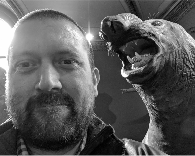
\includegraphics[width=0.45\textwidth]{FIGS/L08-plot-image-svd-original-1.png}
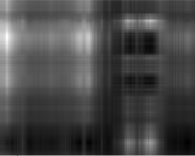
\includegraphics[width=0.45\textwidth]{FIGS/L08-plot-image-svd-n2-1.png}
\end{center}
\vfill
Uses 0.56\% of the original information
\end{frame}



\begin{frame}\frametitle{Using $n=5$ singular values}
\begin{center}
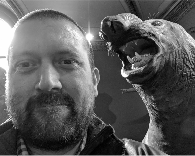
\includegraphics[width=0.45\textwidth]{FIGS/L08-plot-image-svd-original-1.png}
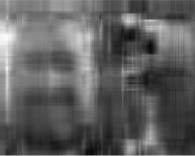
\includegraphics[width=0.45\textwidth]{FIGS/L08-plot-image-svd-n5-1.png}
\end{center}
\vfill
Uses 1.41\% of the original information
\end{frame}




\begin{frame}\frametitle{Using $n=10$ singular values}
\begin{center}
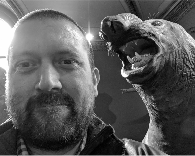
\includegraphics[width=0.45\textwidth]{FIGS/L08-plot-image-svd-original-1.png}
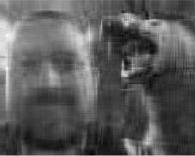
\includegraphics[width=0.45\textwidth]{FIGS/L08-plot-image-svd-n10-1.png}
\end{center}
\vfill
Uses 2.81\% of the original information
\end{frame}





\begin{frame}\frametitle{Using $n=20$ singular values}
\begin{center}
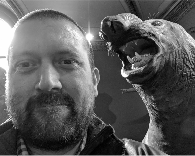
\includegraphics[width=0.45\textwidth]{FIGS/L08-plot-image-svd-original-1.png}
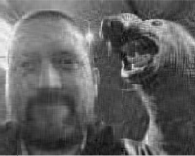
\includegraphics[width=0.45\textwidth]{FIGS/L08-plot-image-svd-n20-1.png}
\end{center}
\vfill
Uses 5.63\% of the original information
\end{frame}





\begin{frame}\frametitle{Using $n=50$ singular values}
\begin{center}
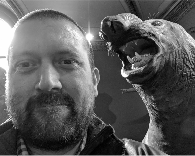
\includegraphics[width=0.45\textwidth]{FIGS/L08-plot-image-svd-original-1.png}
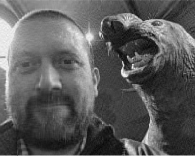
\includegraphics[width=0.45\textwidth]{FIGS/L08-plot-image-svd-n50-1.png}
\end{center}
\vfill
Uses 14.07\% of the original information
\end{frame}





% Save counters for next file

% Save theorem count for next file
\end{document}
